\documentclass[
	12pt, % Default font size, values between 10pt-12pt are allowed
	%letterpaper, % Uncomment for US letter paper size
	%spanish, % Uncomment for Spanish
]{fphw}

% Template-specific packages
\usepackage[utf8]{inputenc} % Required for inputting international characters
\usepackage[T1]{fontenc} % Output font encoding for international characters
\usepackage{mathpazo} % Use the Palatino font

\usepackage{graphicx} % Required for including images
\usepackage{booktabs} % Required for better horizontal rules in tables

\usepackage{listings} % Required for insertion of code

\usepackage{enumerate} % To modify the enumerate environment

\usepackage{amsmath}

\usepackage{subcaption}

\usepackage{hyperref}
\hypersetup{hypertex=true,
colorlinks=true,
linkcolor=blue,
anchorcolor=blue,
citecolor=blue}

%----------------------------------------------------------------------------------------
%	ASSIGNMENT INFORMATION
%----------------------------------------------------------------------------------------

\title{Computational Project} % Assignment title

\author{Junbiao Li} % Student name

% \date{March 28th, 2022} % Due date

\institute{University of Leicester} % Institute or school name

\class{MA2252 Introduction to Computing} % Course or class name

% \professor{Dr. Albert Einstein} % Professor or teacher in charge of the assignment

%----------------------------------------------------------------------------------------

\begin{document} 

\maketitle % Output the assignment title, created automatically using the information in the custom commands above

%----------------------------------------------------------------------------------------
%	ASSIGNMENT CONTENT
%----------------------------------------------------------------------------------------
\begin{problem}
	\textbf{DECLARATION} \\
	All sentences or passages quoted in this Project Report from other people's work have been specifically acknowledged by clear and specific cross referencing to author, work and page(s), or website link. I understand that failure to do so amounts to plagiarism and will be considered grounds for failure in this module and the degree as a whole.\\
	Name: Junbiao Li\\
	Signed: Junbiao Li\\
	Date: March 28th, 2022
\end{problem}

\section*{Topic 1}


%------------------------------------------------

\subsection*{Answer}

In order to get the second order accurate forward, backward and centered finite difference
schemes for finding the derivative. We first write down the Taylor series expansions of $f(x+h)$, $f(x-h)$, $f(x+2h)$,  $f(x-2h)$, $f(x+3h)$ and $f(x-3h)$
\[
\begin{aligned}
f(x+h) &=f(x)+h\frac{f'(x)}{1 !}+h^2 \frac{f''(x)}{2 !} \\
f(x-h) &=f(x)-h\frac{f'(x)}{1 !}+h^2 \frac{f''(x)}{2 !} \\
f(x+2h) &=f(x)+2h\frac{f'(x)}{1 !}+4h^2 \frac{f''(x)}{2 !} \\
f(x-2h) &=f(x)-2h\frac{f'(x)}{1 !}+4h^2 \frac{f''(x)}{2 !} \\
f(x+3h) &=f(x)+3h\frac{f'(x)}{1 !}+9h^2 \frac{f''(x)}{2 !} \\
f(x-3h) &=f(x)-3h\frac{f'(x)}{1 !}+9h^2 \frac{f''(x)}{2 !} \\
\end{aligned}
\]

For the second order accurate forward difference, 
we want to find out $f'(x)=\frac{1}{h}(a_0f(x)+a_1f(x+h)+a_2f(x+2h)+O(h^3))$ 
where $a_0$, $a_1$, $a_2$ are all constant.
Hence, we have
\[
\begin{aligned}
\frac{f'(x)}{1 !} = f'(x)= \frac{1}{h}(&a_0 f(x)+\\
& a_1 f(x)+a_1 f'(x) h+a_1 f''(x) h^2 \\
&a_2 f(x)+2 a_2 f'(x) h+4 a_2 f''(x) h^2 + O(h^3))
\end{aligned}
\]
Which is equivalent to solve a linear system
\[
\left(
	\begin{array}{ccc|c}
	1 & 1 & 1 & 0 \\
	0 & 1 & 2 & 1 \\
	0 & 1 & 4 & 0 \\
	\end{array}
\right)
\]

Hence, $a_0 = -\frac{3}{2}$, $a_1=2$ and $a_3 = -\frac{1}{2}$, and 
\[f' (x)=\frac{-\frac{3}{2}f (x)+2f (x+h) -\frac{1}{2}f (x+2h)}{h}+O(h^2)\]

With the same process, We can calculate second order accurate forward, backward and centered finite difference
schemes for first derivative and second derivative:
\begin{enumerate}
\item Second order accurate centered difference approximations:
\[
\begin{aligned}
f' (x): & (f (x+h)-f (x-h)) /(2 h) \\
f'' (x): & (f (x+h)-2 f (x)+f (x-h)) / h^2
\end{aligned}
\]
\item Second order accurate forward difference approximations:
\[
\begin{aligned}
f' (x): & (-3 f (x)+4 f (x+h)-f (x+2 h)) / (2 h) \\
f'' (x): & (2 f (x)-5 f (x+h)+4 f (x+2 h)-f (x+3 h)) / h^2
\end{aligned}
\]
\item Second order accurate backward difference approximations:
\[
\begin{aligned}
f' (x): & (3 f (x)-4 f (x-h)+f (x-2 h)) / (2 h) \\
f'' (x): & (2 f (x)-5 f (x-h)+4 f (x-2 h)-f (x-3 h)) / h^2
\end{aligned}
\]
\end{enumerate}

\subsection*{Implement}

I chose $x^4+\sin(x)$ as test function, with $0\leq x \leq 2$ and $h=0.1$

\begin{figure}[h!]
	\centering
	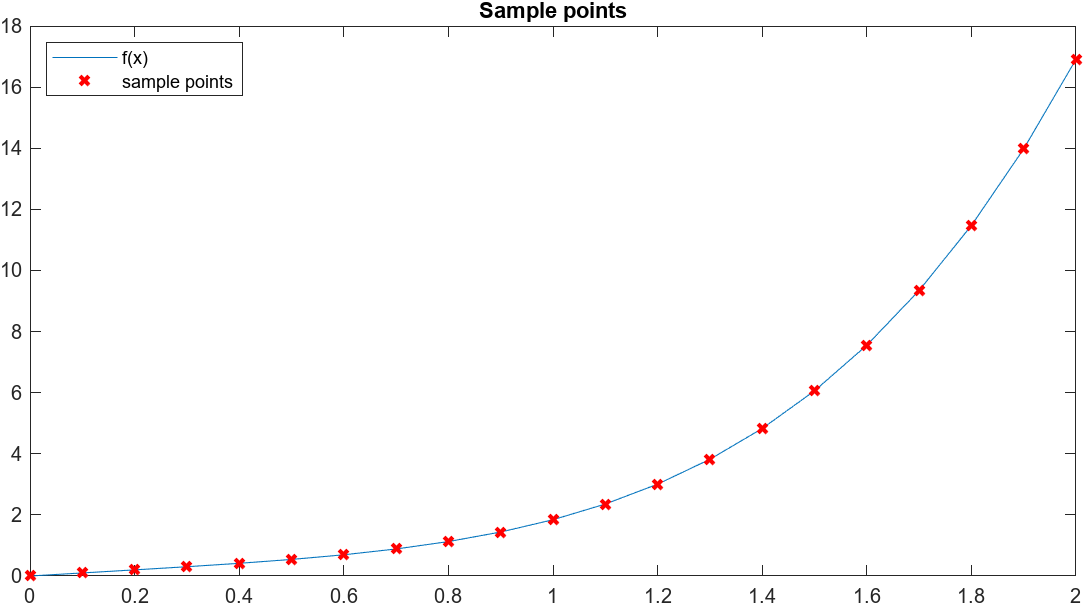
\includegraphics[width=0.8\columnwidth]{img/sample_points.png} % Example image
	\caption{Sample Points of f(x)}
	\label{fig:sample_points}
\end{figure}

After applying second order accurate difference approximations, I draw $f'(x)$ and $f''(x)$ to check the difference between real derivative and finite difference schemes.

\begin{figure}[h!]
	\centering
	\begin{subfigure}[b]{0.4\linewidth}
	  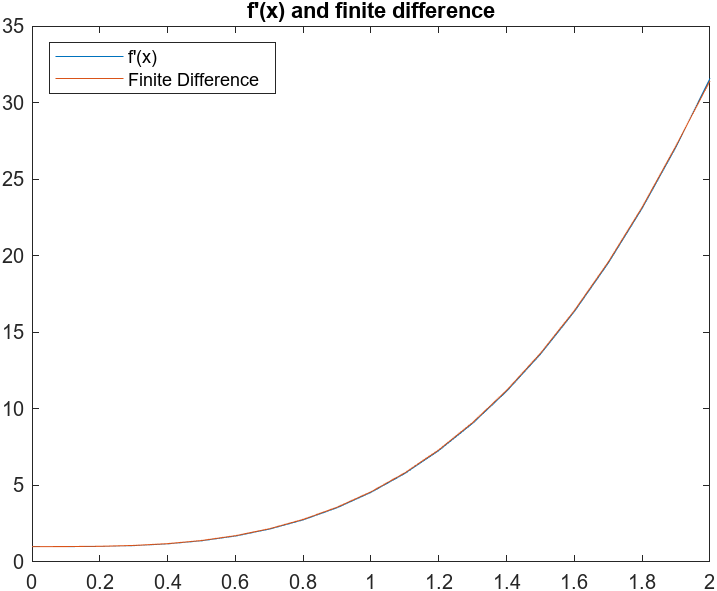
\includegraphics[width=\linewidth]{img/f'(x).png}
	  \caption{f'(x)}
	\end{subfigure}
	\begin{subfigure}[b]{0.4\linewidth}
	  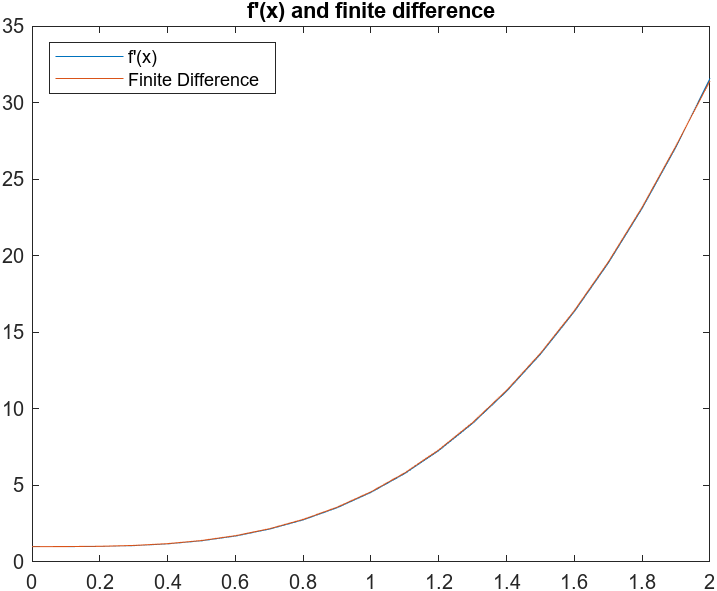
\includegraphics[width=\linewidth]{img/f'(x).png}
	  \caption{f''(x)}
	\end{subfigure}
	\caption{Compare real derivative and finite difference}
	\label{fig:compare}
\end{figure}

Figure.\ref{fig:compare} told us that the second order accurate difference approximations is really close to the real derivative, even their actually difference. You can find more implement detail in the code. 
%----------------------------------------------------------------------------------------

\section*{Topic 2}

\subsection*{Answer}

In order to evaluate double integrals which is perform on the rectangle $R = \{ (x, y) \in \mathbb{R}^2: a \leq x \leq b and c \leq y \leq d  \} $, We first consider the uniform-grid in each 
dimension. Let grid space of $x$ and $y$ be the $h$, which means we have $x_1, x_2, \cdots , x_{n_x}$ and $y_1, y_2, \cdots , y_{n_y}$.

\subparagraph*{Task 1}
Now  apply trapezoidal rule to calculate the integral with respect to $x$ with fixed $y$.
\[
\begin{aligned} \label{g(y)}
g(y) &= \int^{b}_{a}f(x,y)\,dx \\
	 &= \sum^{n_x-1}_{i=1}\frac{1}{2}[f(x_i)+f(x_{i+1})]h \\
	 &= \frac{h}{2} [f(x_0, y) + f(x_{n_x}, y) + 2\sum^{n_x-1}_{i=2}f(x_i, y)] \\
	 &= \frac{h}{2} [f(a, y) + f(b, y) + 2\sum^{n_x-1}_{i=2}f(x_i, y)] 
\end{aligned}
\]
Finally we get $g(y)=\frac{h}{2} [f(a, y) + f(b, y) + 2\sum^{n_x}_{i=2}f(x_i, y)]$

\subparagraph*{Task 2}
After integrate $x$, we now integrate $y$, 
\[
\begin{aligned} \label{I}
I &= \int^{d}_{c}g(y)\,dy \\
%   &= \int^{d}_{c}\frac{h}{2} [f(a, y) + f(b, y) + 2\sum^{n_x-1}_{i=2}f(x_i, y)] \,dy \\
  &= \sum^{n_y}_{i=1}\frac{1}{2} [g(y_i)+g(y_{i+1})]h \\
  &= \frac{h}{2} [g(c) + g(d) + 2\sum^{n_y}_{i=2}g(y_i)+g(y_{i+1})]
\end{aligned}
\]
Substituting \ref{g(y)} into  \ref*{I}
\[
\begin{aligned}
I = \frac{h}{2}\{&\frac{h}{2}[f(a, c) + f(b, c) + 2\sum^{n_x}_{i=2}f(x_i, c)]	\\
	 			+&\frac{h}{2}[f(a, d) + f(b, d) + 2\sum^{n_x}_{i=2}f(x_i, d)]	\\
	 			+&\frac{h}{2}[f(a, y) + f(b, y) + 2\sum^{n_x}_{i=2}f(x_i, y)]\}	
\end{aligned}
\]

\end{document} 